\documentclass[11pt,aspectratio=169]{beamer}

\usetheme{Singapore}
\usecolortheme{orchid}

\usepackage[utf8]{inputenc}
\usepackage[russian]{babel}
\usepackage{amsmath}
\usepackage{amsfonts}
\usepackage{amssymb}
\usepackage{graphicx}
\usepackage{bibentry}
\usepackage{wasysym}
\usepackage[most]{tcolorbox}
\usepackage[normalem]{ulem}

\usepackage{hyperref}

\definecolor{info}{RGB}{62, 180, 137}
\definecolor{warn}{RGB}{128, 0, 0}

\author{Николай Анохин}
\title{Классические алгоритмы рекомендаций}

\logo{
\includegraphics[width=.05\textwidth]{images/ok_logo.png}}

\AtBeginSection[]{
  \begin{frame}
  \vfill
  \centering
  \begin{beamercolorbox}[sep=8pt,center,shadow=true,rounded=true]{title}
    \usebeamerfont{title}\insertsectionhead\par
  \end{beamercolorbox}
  \vfill
  \end{frame}
}

\begin{document}

{
\setbeamertemplate{headline}{}

\begin{frame}
\titlepage
\end{frame}

%\begin{frame}
%\tableofcontents
%\end{frame}

}

\begin{frame}{Контекст}

\begin{center}
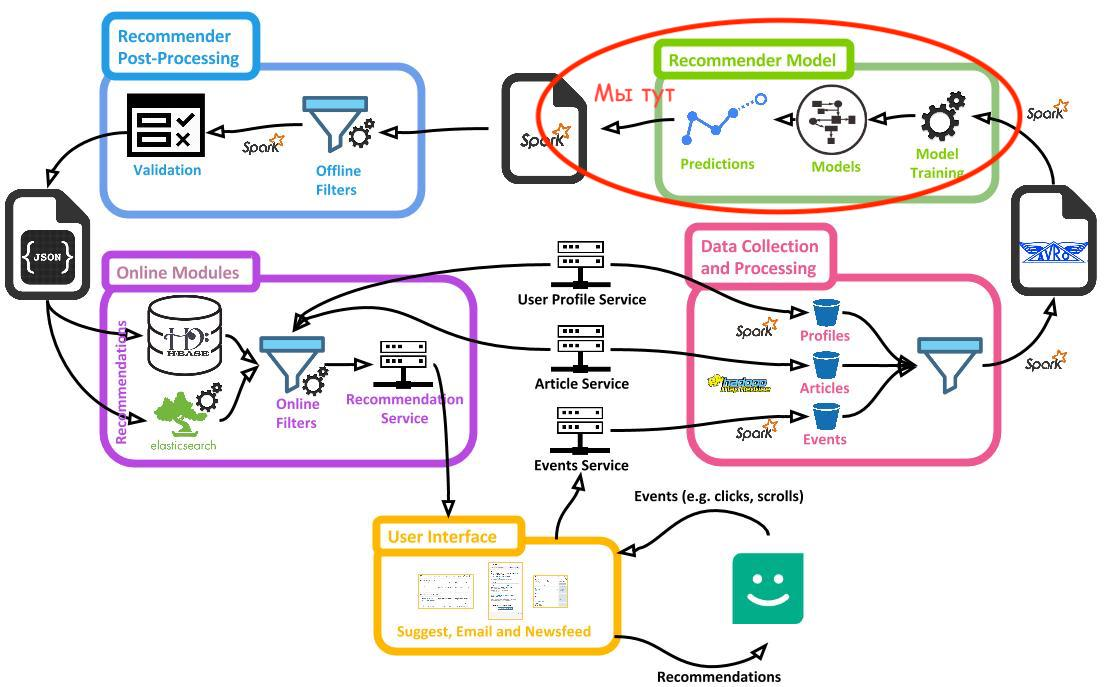
\includegraphics[scale=0.23]{images/mendeley.jpeg}
\end{center}

\end{frame}

\begin{frame}
\begin{center}
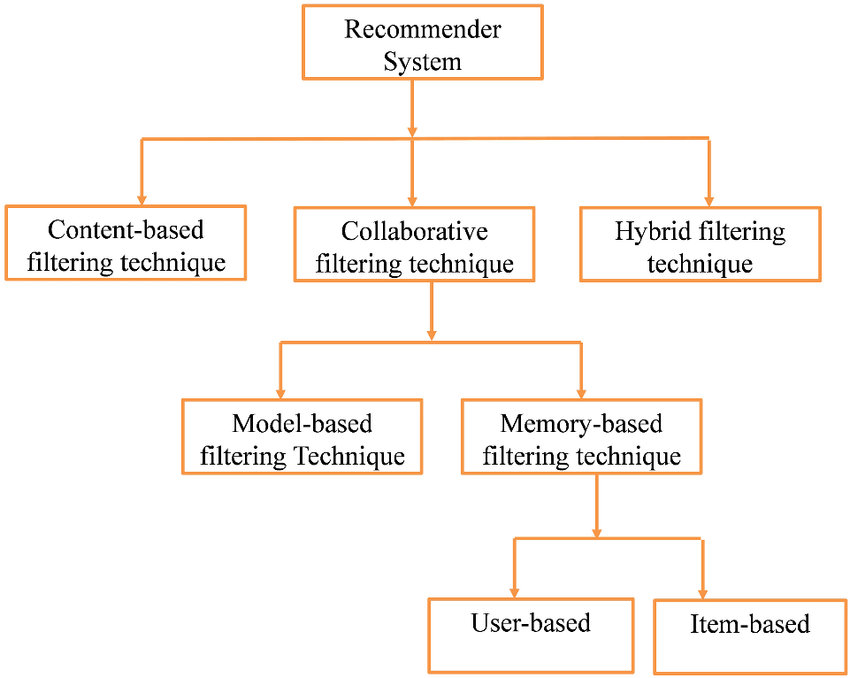
\includegraphics[scale=0.22]{images/taxonomy.png}
\end{center}
\end{frame}

\section{Content-based RS}

\begin{frame}{Пример: интуиция}

\begin{columns}

\begin{column}{0.47\textwidth} 

Нравится:
\begin{itemize}
\item Возвращение короля
\item Король былого и грядущего
\item Война мага
\end{itemize}

Не нравится:
\begin{itemize}
\item Новый ум короля
\end{itemize}

Что порекомендуем?
\begin{itemize}
\item Битва королей
\item Война и мир
\end{itemize}

\end{column}

\begin{column}{0.47\textwidth} 

\end{column}

\end{columns}

\end{frame}

\begin{frame}{Content-based RS}

\begin{columns}

\begin{column}{0.47\textwidth} 
\begin{tcolorbox}[colback=info!5,colframe=info!80,title=Идея]
Рекомендуем пользователю айтемы, похожие на те, что нравились ей раньше
\end{tcolorbox}
\end{column}

\begin{column}{0.47\textwidth} 
\begin{center}
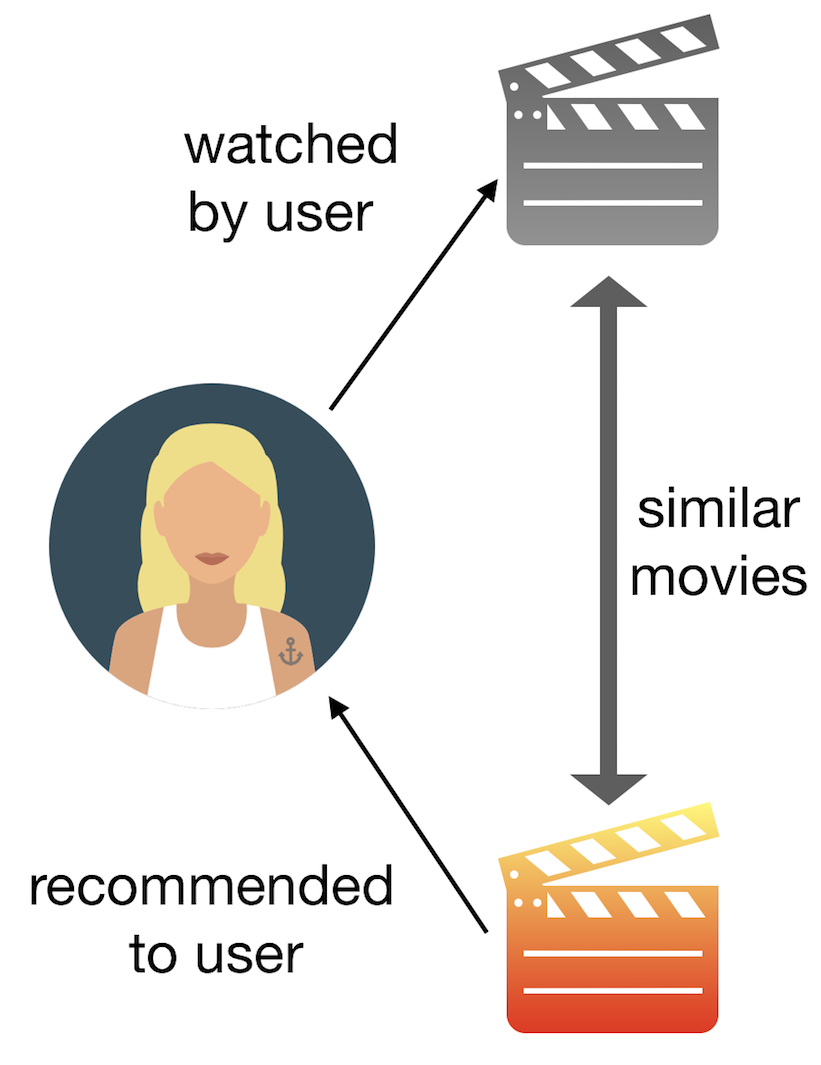
\includegraphics[scale=0.15]{images/content-idea.png}
\end{center}
\end{column}

\end{columns}

\end{frame}

\begin{frame}{Архитектура CBRS \cite{RSHB}}

\begin{center}
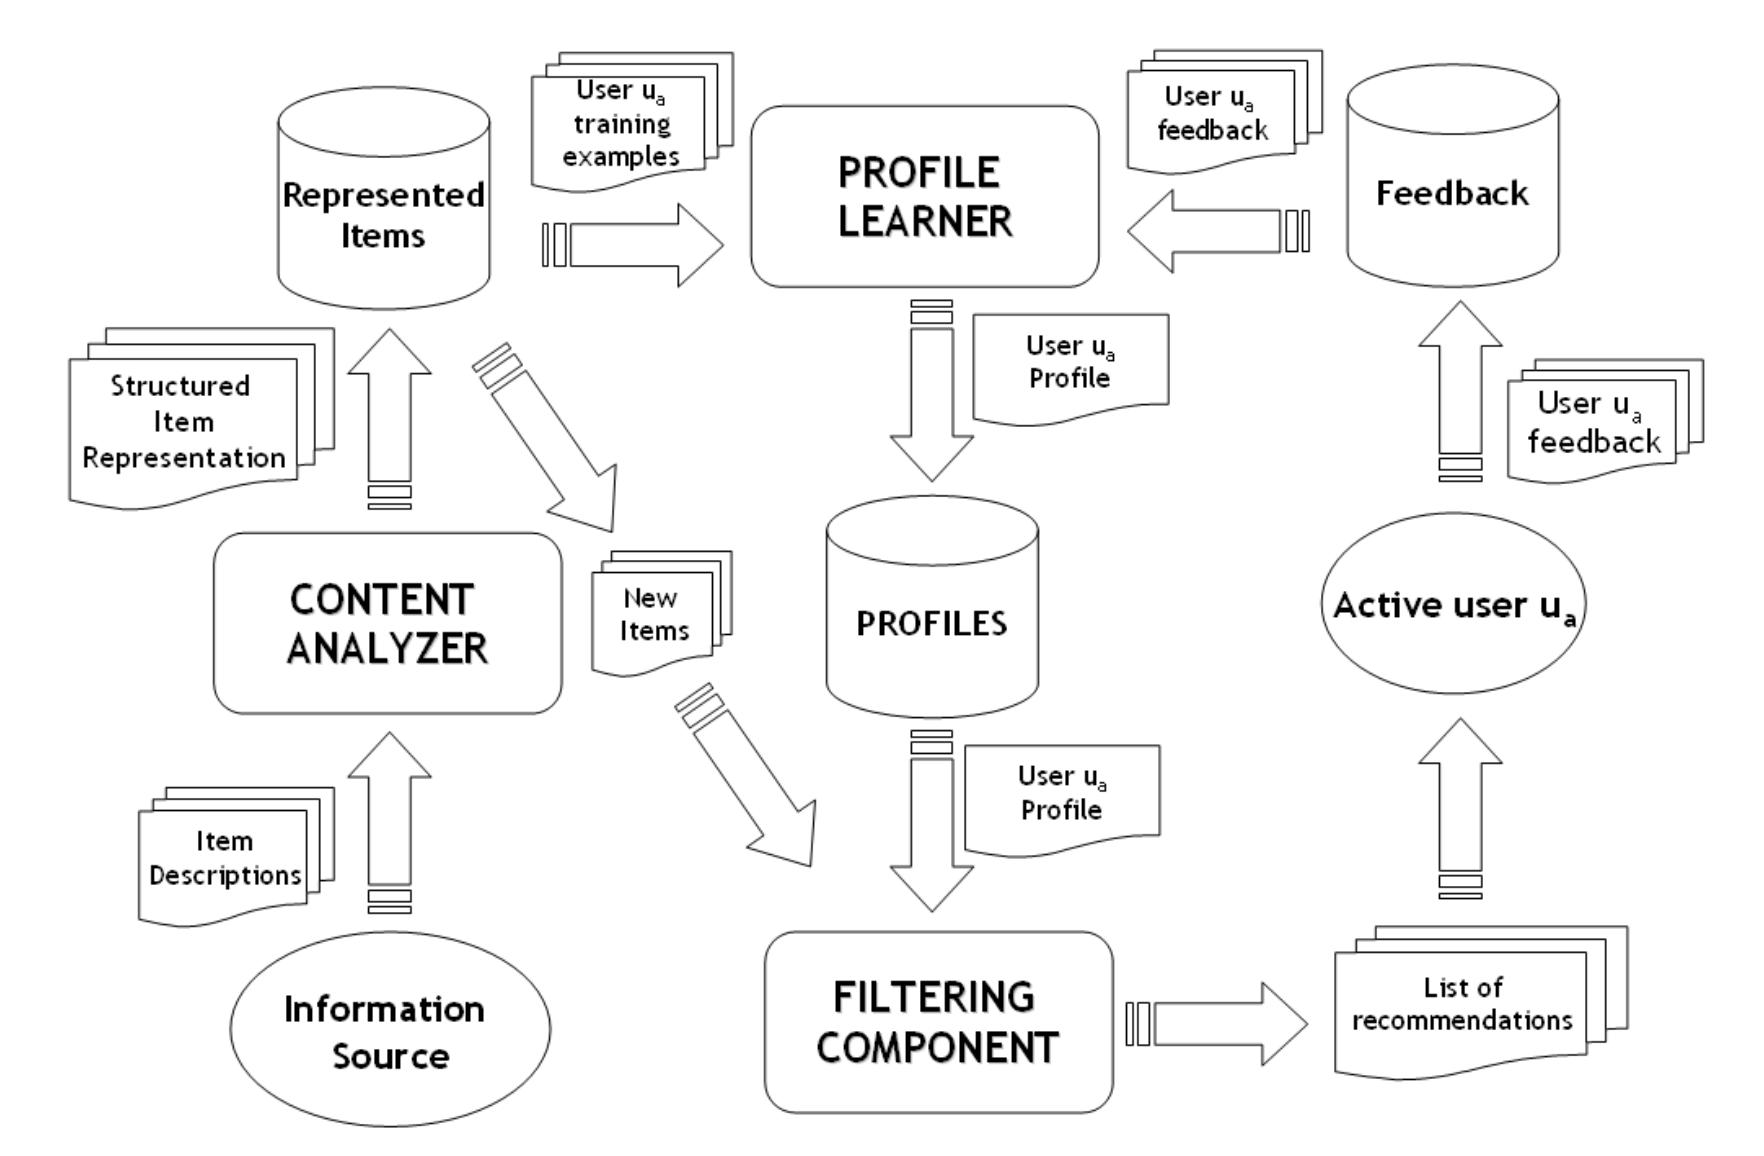
\includegraphics[scale=0.3]{images/cbf.png}
\end{center}

\end{frame}

\begin{frame}{Анализ контента}

\begin{center}
\begin{tabular}{ l | p{20em} }
{\bf Данные} & {\bf Признаки} \\
\hline
Табличные \pause &  Категориальные / числовые \\
Текст \pause & BOW / TF-IDF / BM25 / NN Эмбеддинги \\
Картинки \pause & SIFT / SURF / NN Эмбеддинги \\
Музыка \pause & Spectral 
\end{tabular}
\end{center}

\end{frame}

\begin{frame}{Supervised профили пользователей}

\begin{columns}
\begin{column}{0.15\textwidth} 
\end{column}
\begin{column}{0.6\textwidth} 
\begin{tcolorbox}[colback=info!5,colframe=info!80,title=Модель]
\[
p(u \, likes \, i) = f(x_i, x_u, \theta)
\]
\[
recommendations = \arg_i topk \, p(u \, likes \, i)
\]
\end{tcolorbox}
\end{column}
\begin{column}{0.15\textwidth} 
\end{column}
\end{columns}

\vfill

\begin{columns}
\begin{column}{0.45\textwidth}   
   Обучаемые параметры:
  \begin{itemize}
    \item $x_u$ -- профиль пользователя
    \item $\theta$ -- параметры модели
  \end{itemize}
  
  Данные:
  \begin{itemize}
    \item $\left\{ (x_i, u_j \, likes \, x_i) \right\}^N$
  \end{itemize}

\end{column}

\begin{column}{0.45\textwidth}
  Примеры моделей:
  \begin{itemize}
  \item Naive Bayes
  \item Rocchio
  \item Meta-learning
  \end{itemize}
    
\end{column}
\end{columns}

\end{frame}

\begin{frame}{Unsupervised профили пользователей}

\begin{tcolorbox}[colback=info!5,colframe=info!80,title=Идея]
Храним айтемы, с которыми взамиодействовал пользователь, и рекомендуем ближайшие к ним.
\end{tcolorbox}

\vfill

Когда айтемов у пользователя слишком много:
\begin{itemize}
\item Храним последние
\item Кластеризуем и храним представления кластеров \cite{PINNERSAGE}
\end{itemize} 

\end{frame}

\begin{frame}{Пример: формально}

\begin{columns}

\begin{column}{0.47\textwidth} 

Нравится:
\begin{itemize}
\item Возвращение короля
\item Король былого и грядущего
\item Война мага
\end{itemize}

Не нравится:
\begin{itemize}
\item Новый ум короля
\end{itemize}

Что порекомендуем?
\begin{enumerate}
\item Битва королей
\item Война и мир
\end{enumerate}

\end{column}

\begin{column}{0.47\textwidth}
\begin{footnotesize}
Naive Bayes
\[
p(c | d) \sim p(c) p(d | c) = 
\]
\[
= p(c) \prod_j p(w_j | c) \sim \log p(c) + \sum_j \log p(w_j | c)
\]
\[
p(w_j | c) = \frac{N_{jc} + \alpha}{N_c + \alpha |V|}
\]
% возвращение король былое грядущее война маг новый ум битва мир
Размер словаря $|V| = 10$, $\alpha = 1$ \\
Вероятности классов $p(+) = 3/4$, $p(-) = 1/4$
Скоры документов
\[
p(+|1) \sim \log 3/4 + \log 1 / 13 + \log 3 / 13
\]
\[
p(-|1) \sim \log 1/4 + \log 1 / 11 + \log 2 / 11
\]
\[
s(1) = p^*(+|1)  - p^*(-|1) = 2.69
\]
% s(2) = 2.10
\end{footnotesize}
\end{column}

\end{columns}

\end{frame}

\begin{frame}{Известные использования}

\begin{itemize}
\item Spotify: Deep content-based music recommendation \cite{SPOTIFY}
\item Ozon: Векторное представление товаров Prod2Vec: как мы улучшили матчинг и избавились от кучи эмбеддингов \cite{OZON}
\end{itemize}

\end{frame}

\begin{frame}{Итоги}

\begin{tcolorbox}[colback=info!5,colframe=info!80,title=Плюсы]
  \begin{itemize}
    \item Рекомендации строятся независимо для каждого пользователя
    \item Рекомендации часто можно объяснить
    \item Естественная поддержка холодного старта айтемов
  \end{itemize}
\end{tcolorbox}

\begin{tcolorbox}[colback=warn!5,colframe=warn!80,title=Минусы]
  \begin{itemize}
    \item Полагаются на (несовершенные) техники анализа контента
    \item Нет поддержки холодного старта пользователей
        \item Отсутствие новизны: умеют рекомендовать только похожие айтемы
  \end{itemize}
\end{tcolorbox}

\end{frame}

\section{Neighbourhood-based Collaborative Filtering}

\begin{frame}{Пример: интуиция \cite{MMDS}}

\begin{center}
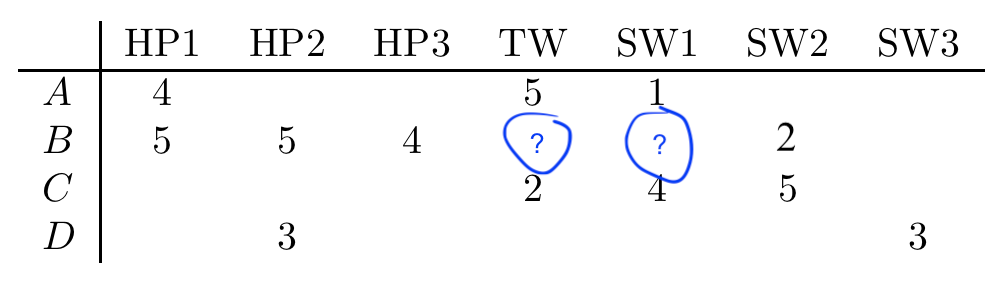
\includegraphics[scale=0.5]{images/utility.png}
\end{center}

\end{frame}

\begin{frame}{Collaborative filtering\footnote{Оскар за худшее название алгоритма}-based RS}

\begin{columns}

\begin{column}{0.47\textwidth} 
\begin{tcolorbox}[colback=info!5,colframe=info!80,title=Идея]
Рекомендуем пользователю айтемы, которые понравились похожим на нее пользователям. Пользователи похожи, если они похоже оценивают одни и те же айтемы.
\end{tcolorbox}
\end{column}

\begin{column}{0.47\textwidth} 
\begin{center}
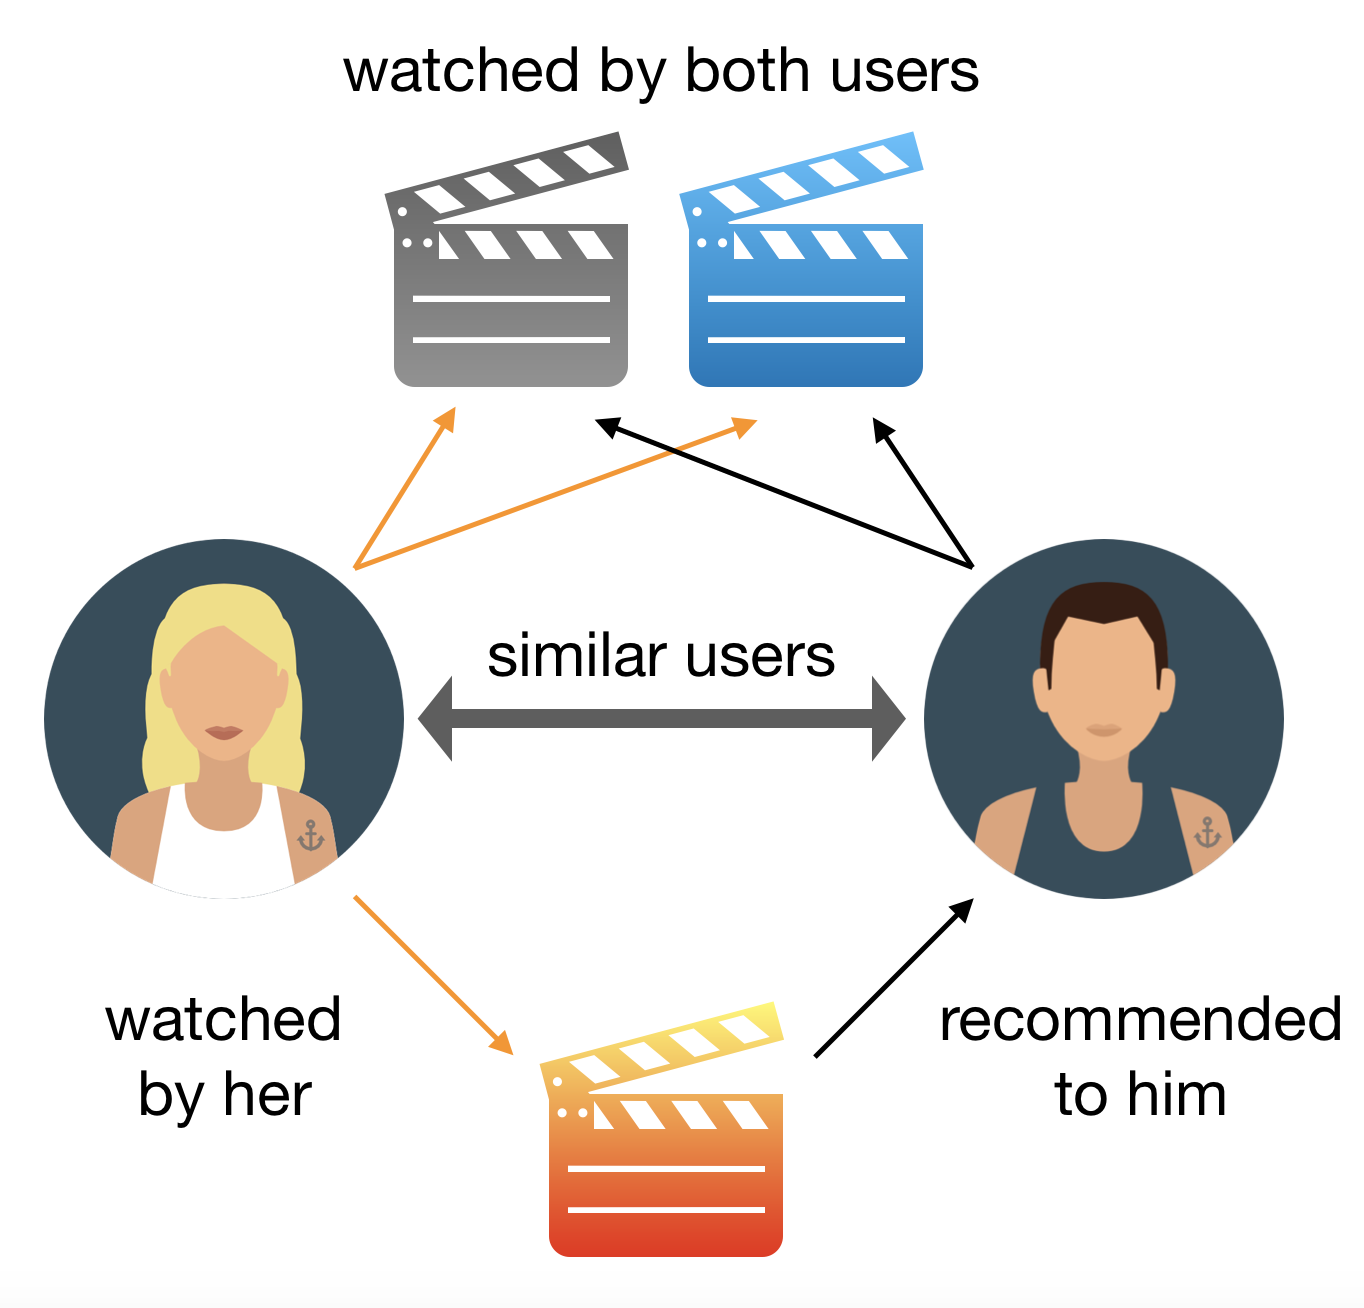
\includegraphics[scale=0.1]{images/cf-idea.png}
\end{center}
\end{column}

\end{columns}

\end{frame}

\begin{frame}

\begin{columns}
\begin{column}{0.45\textwidth}   
\quad\; User-based
   \[
   \hat r_{ui} = h^{-1} \left( \frac{\sum_{v \in N_i(u)} w_{uv} h(r_{vi})}{\sum_{v \in N_i(u)} w_{uv}} \right)
   \]
\end{column}
\begin{column}{0.45\textwidth}
\quad\; Item-based
  \[
  \hat r_{ui} = h^{-1} \left( \frac{\sum_{j \in N_u(i)} w_{ij} h(r_{uj})}{\sum_{j \in N_u(i)} w_{ij}} \right)
  \]
\end{column}
\end{columns}

\vfill

\begin{itemize}
\item $N_i(u)$ -- соседи пользователя $u$, которые оценили айтем $i$
\item $N_u(i)$ -- соседи айтема $i$, которые оценила пользователь $u$
\item $w_{uv}, w_{ij}$ -- веса соседей
\item $h$ -- функция нормализации
\end{itemize}

\end{frame}

\begin{frame}

Как вычислить веса $w_{uv}$, $w_{ij}$?
\[
cos(u, v) = \frac{\sum_{i \in I_{uv}} r_{ui} r_{vi}}{\sqrt{\sum_{i \in I_u} r_{ui}^2 \sum_{i \in I_v} r_{vi}^2}}
\]
\[
pearson(u, v) = \frac{\sum_{i \in I_{uv}} (r_{ui} - \bar r_u) (r_{vi} - \bar r_v)}{\sqrt{\sum_{i \in I_{uv}} (r_{ui} - \bar r_u)^2 \sum_{i \in I_{uv}} (r_{vi}^2 - \bar r_v)}}
\]

\end{frame}

\begin{frame}

{\bf Дано:} \\
100 айтемов \\
1000 пользователей \\
10000 рейтингов равномерно распределены по пользователям и айтемам \\

\vfill

{\bf Вопрос:} \\
Сколько в среднем общих айтемов у пары пользователей? \\
Сколько в среднем общих пользователей у пары айтемов? \\

\vfill

\begin{tcolorbox}[colback=gray!5,colframe=gray!80,title=]
Небольшое количество надежных соседей лучше, чем много ненадежных
\begin{itemize}
\item User-based ($|U| < |I|$)
\item Item-based  ($|U| > |I|$)
\end{itemize}
\end{tcolorbox}

\end{frame}

\begin{frame}

\begin{tcolorbox}[colback=gray!5,colframe=gray!80,title=Locality-Sensitive Hashing для приближенного поиска соседей]
The general idea of LSH is to use a family of functions (“LSH families”) to hash data points into buckets, so that the data points which are close to each other are in the same buckets with high probability, while data points that are far away from each other are very likely in different buckets.
\end{tcolorbox}

\begin{center}
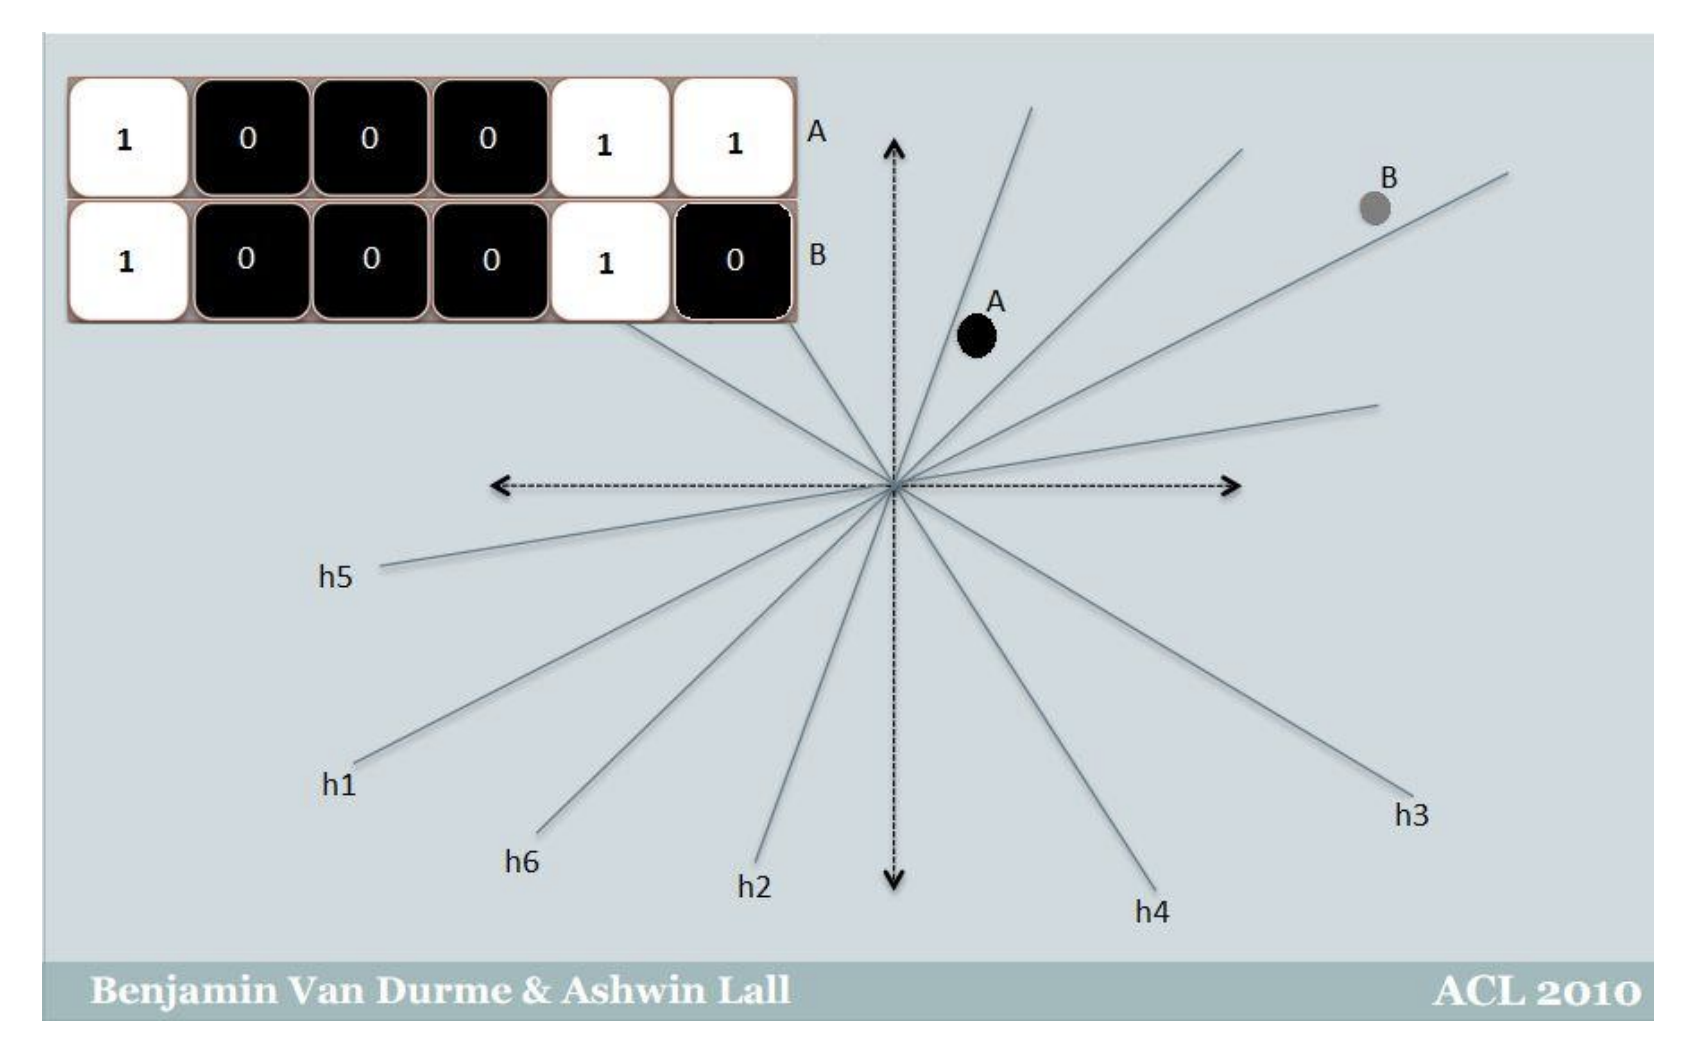
\includegraphics[scale=0.2]{images/lsh.png}
\end{center}

\end{frame}

\begin{frame}{Пример: формально}

\begin{center}
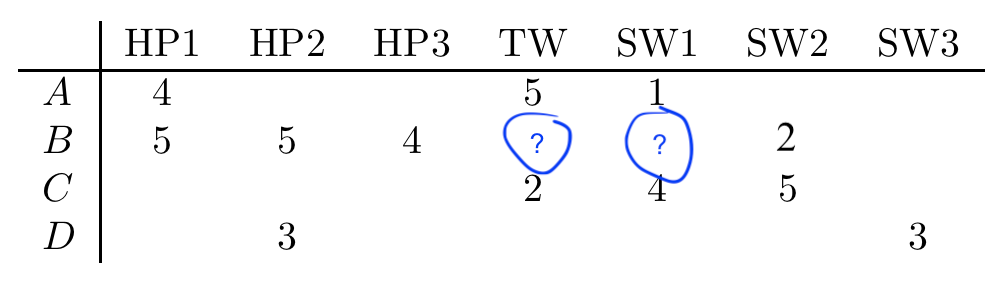
\includegraphics[scale=0.5]{images/utility.png}
\end{center}

Нормализация: $h(r) = r$
Веса
\[
cos(A, B) = \frac{4 \dot 5}{ \sqrt{42} \sqrt{66} } = 0.37
\]
% 0.18
\[
cos(B, C) = \, ? 
\]
% 4.0, 2.0
\[
r(TW) = \, ? \quad r(SW1) = \, ?
\]

\end{frame}

\begin{frame}{}

\begin{tcolorbox}[colback=info!5,colframe=info!80,title=Плюсы]
  \begin{itemize}
    \item Простота и интуитивность: рекомендации можно объяснить.
    \item Небольшое количество параметров
    \item Не нужно обучать, удобно добавлять новых пользователей и айтемы
  \end{itemize}
\end{tcolorbox}

\begin{tcolorbox}[colback=warn!5,colframe=warn!80,title=Минусы]
  \begin{itemize}
    \item User-based: очень много пользователей для поиска NN
    \item Item-based: как понять, для каких айтемов считать рейтинги?
    \item Разреженность пространства
  \end{itemize}
\end{tcolorbox}

\end{frame}

\section{Model-based Collaborative Filtering}

\begin{frame}{Model-based CF}

\begin{tcolorbox}[colback=info!5,colframe=info!80,title=Идея]
Выучим модель, которая поможет заполнить ``пробелы'' в user-item матрице.
\end{tcolorbox}

\begin{center}
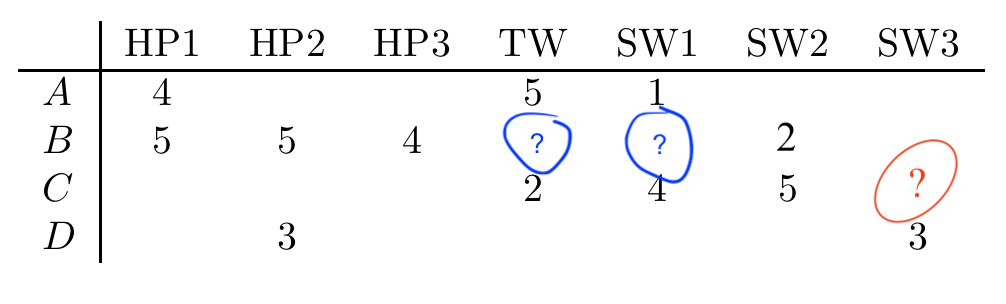
\includegraphics[scale=0.5]{images/utility-2.png}
\end{center}

\end{frame}

\begin{frame}{Бейзлайн \cite{KOREN}}

\begin{columns}
\begin{column}{0.2\textwidth} 
\end{column}
\begin{column}{0.5\textwidth} 
\begin{tcolorbox}[colback=info!5,colframe=info!80,title=Модель]
\[
b_{ui} = \mu + b_u + b_i
\]
\end{tcolorbox}
\end{column}
\begin{column}{0.2\textwidth} 
\end{column}
\end{columns}

\vfill

\begin{itemize}
\item $\mu$ -- средний рейтинг
\item $b_u$ -- bias пользователя
\item $b_i$ -- bias айтема
\end{itemize}

\vfill

Оптимизируем
\[
\sum_{u, i} (b_{ui} - \mu - b_u - b_i)^2 + \lambda_1 b_u^2 + \lambda_2 b_i^2 \rightarrow min_{b_u, b_i}
\]

\end{frame}

\begin{frame}{SVD}

\begin{columns}
\begin{column}{0.2\textwidth} 
\end{column}
\begin{column}{0.5\textwidth} 
\begin{tcolorbox}[colback=info!5,colframe=info!80,title=Модель]
\[
\hat r_{ui} = \mu + b_u + b_i + q_i^T p_u
\]
\end{tcolorbox}
\end{column}
\begin{column}{0.2\textwidth} 
\end{column}
\end{columns}

\vfill

\begin{itemize}
\item $q_i$ -- латентное представление айтема
\item $p_u$ -- латентное представление пользователя
\end{itemize}

\vfill

Оптимизируем
\[
\sum_{u, i} (r_{ui} - \mu - b_u - b_i - q_i^T p_u)^2 + \lambda (b_u^2 +  b_i^2 + \| q_i \|^2 + \| p_u \|^2) \rightarrow min_{b_u, b_i, p_u, q_i}
\]

\end{frame}

\begin{frame}
\begin{center}
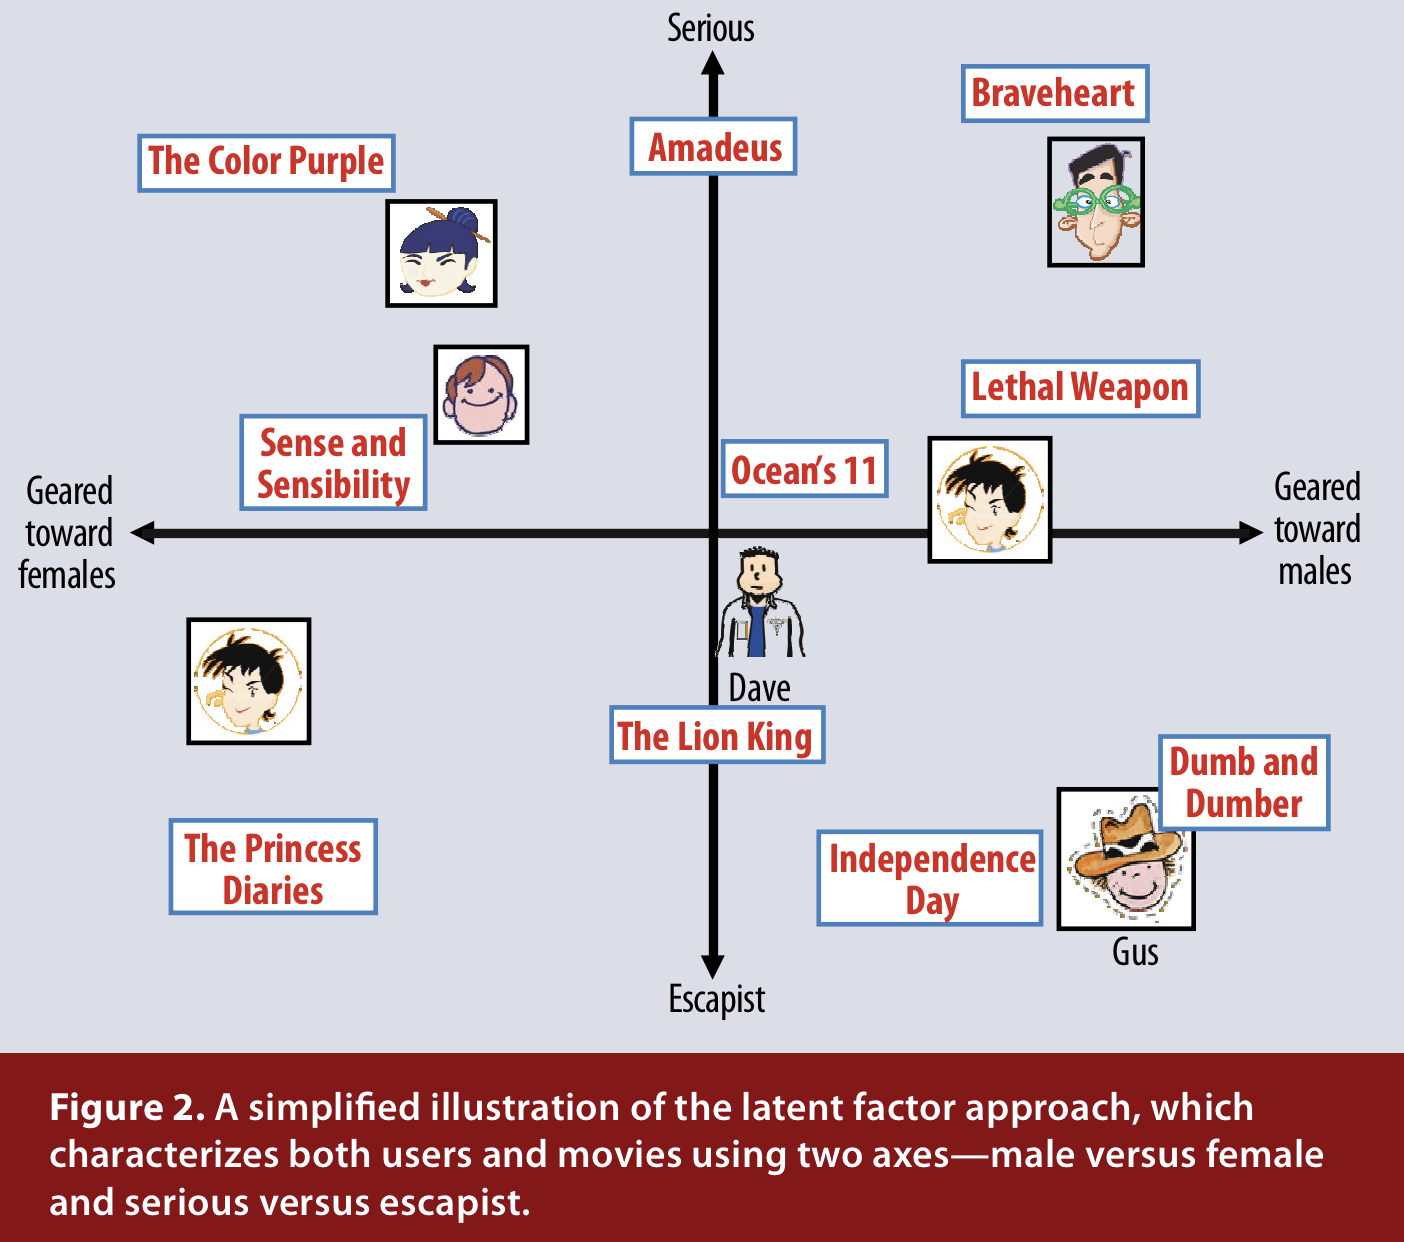
\includegraphics[scale=0.3]{images/latent.png}
\end{center}
\end{frame}

\begin{frame}{Как оптимизировать}
\[
\sum_{u, i} (r_{ui} - \mu - b_u - b_i - q_i^T p_u)^2 + \lambda (b_u^2 +  b_i^2 + \| q_i \|^2 + \| p_u \|^2)
\]

\begin{itemize}
\item ALS \cite{IMPLICIT}
% Линейное врем по N!
\begin{enumerate}
\item фиксируем $p_u, b_u$, оптимизируем $q_i, b_i$ -- получем линрег 1
\item фиксируем  $q_i, b_i$, оптимизируем $p_u, b_u$ -- получем линрег 2
\item повторяем до сходимости
\end{enumerate}
\item SGD
\end{itemize}

\end{frame}

\begin{frame}{SVD++}

\begin{columns}
\begin{column}{0.1\textwidth} 
\end{column}
\begin{column}{0.7\textwidth} 
\begin{tcolorbox}[colback=info!5,colframe=info!80,title=Модель]
\[
\hat r_{ui} = \mu + b_u + b_i + q_i^T \left( p_u + \frac{1}{\sqrt{|R(u)|}} \sum_j y_j \right)
\]
\end{tcolorbox}
\end{column}
\begin{column}{0.1\textwidth} 
\end{column}
\end{columns}

\vfill

\begin{itemize}
\item $y_i$ -- латентное представление айтемов, на которые пользователь дал implicit feedback до оценки айтема $i$
\end{itemize}

\end{frame}

\begin{frame}{Time SVD++}

\begin{tcolorbox}[colback=info!5,colframe=info!80,title=Модель]
\[
\hat r_{ui} = \mu + b_u(t_{ui}) + b_i(t_{ui}) + q_i^T \left( p_u(t_{ui}) + \frac{1}{\sqrt{|R(u)|}} \sum_j y_j \right)
\]
\end{tcolorbox}

\vfill

\begin{itemize}
\item $t_{ui}$ -- время, когда пользователь оценил айтем
\end{itemize}

\end{frame}

\begin{frame}{Netflix Prize }

\begin{center}
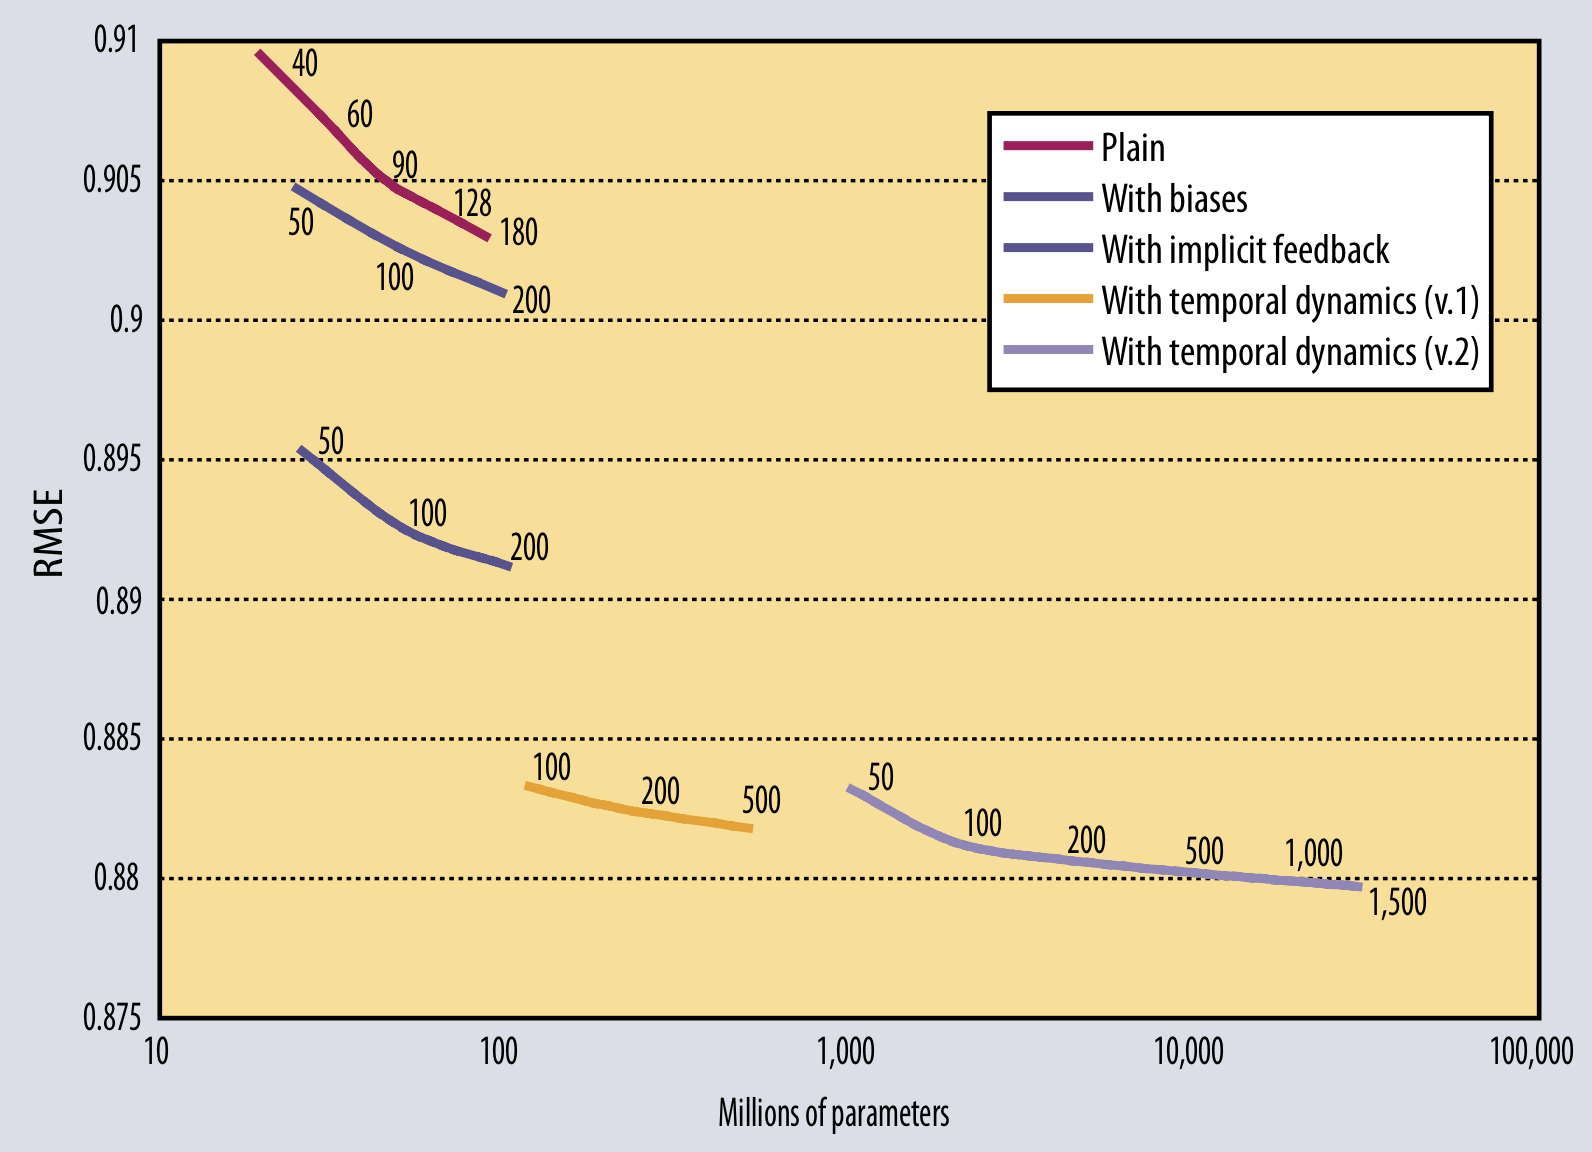
\includegraphics[scale=0.25]{images/svd-compare.png}
\end{center}

\begin{small}
September 21, 2009, the grand prize of US\$1,000,000 was given to the BellKor's Pragmatic Chaos team which bested Netflix's own algorithm for predicting ratings by 10.06
\end{small}

\end{frame}

\begin{frame}{LightFM \cite{LIGHT}}

\begin{tcolorbox}[colback=info!5,colframe=info!80,title=Модель]
\[
\hat r_{ui} = \mu + b_u + b_i + q_i^T p_u
\]
\[
q_i = \sum_{j \in f_i} v_j, \quad p_u = \sum_{j \in f_u} w_j
\]
\end{tcolorbox}

\vfill

\begin{itemize}
\item $f_i$ -- признаки айтема
\item $v_j$ -- латентное представление признаков айтема
\item $f_u$ -- признаки пользователя
\item $w_j$ -- латентное представление признаков пользователя
\end{itemize}

\end{frame}

\begin{frame}{Альтернативные loss-функции: classification vs regression}

\begin{tcolorbox}[colback=info!5,colframe=info!80,title=]
Случай implicit feedback похож скорее на задачу классификации, чем регресии
\end{tcolorbox}

\[
\hat p_{ui}(r=1) = \sigma(\mu + b_u + b_i + q_i^T p_u)
\]

Лосс: кросс-энтропия

\end{frame}

\begin{frame}{Альтернативные loss-функции: ranking with BPR \cite{BPR}}

\begin{tcolorbox}[colback=info!5,colframe=info!80,title=]
Правильное ранжирование важнее, чем точное предсказание рейтинга / фидбэка
\end{tcolorbox}

\[
\hat p(u \, prefers \, i \, to \, j) = \sigma(\hat x_{uij}) = \sigma(\hat x_{ui} - \hat x_{uj})
\]
Лосс:
\[
- \sum \log p(u \, prefers \, i \, to \, j) + \lambda \| \theta \|^2
\]

\end{frame}

\begin{frame}{Альтернативные loss-функции: WARP \cite{WARP}}

\begin{tcolorbox}[colback=info!5,colframe=info!80,title=]
Можно умно семплировать негативные примеры -- так, чтобы сложность негативных примеров увеличивалась, когда модель становится точнее.
\end{tcolorbox}

Дано: пользователь + позитивный айтем
\begin{enumerate}
\item Семплируем негативные, пока не найдем неправильно отранжированную пару. Делаем шаг обновления.
\item Чем больше пришлось семплировать, тем меньше learning rate шага обновления.
\end{enumerate}

\end{frame}

\begin{frame}{Реализации}

\begin{center}
\begin{tabular}{l c c c}
 & Spark & LightFM & Implicit \\
\hline
\hline
SGD & & \checked & \\
ALS & \checked & & \checked \\
\hline
RMSE & \checked &  & \checked \\
logistic & & \checked & \checked \\
BPR & & \checked & \checked \\
WARP & & \checked & \\
\hline
GPU & & & \checked \\
\end{tabular}
\end{center}

\end{frame}

\begin{frame}{}

\begin{tcolorbox}[colback=info!5,colframe=info!80,title=Плюсы]
  \begin{itemize}
    \item Качество рекомендаций: новизна как у neighbourhood-based CF, но можно заполнить все пробелы в user-item матрице
    \item Большой выбор моделей и лоссов
    \item Можно переформулировать как нейронную сеть
  \end{itemize}
\end{tcolorbox}

\begin{tcolorbox}[colback=warn!5,colframe=warn!80,title=Минусы]
  \begin{itemize}
    \item Сложные алгоримы оптимизации
    \item Холодный старт как пользователей, так и айтемов нужно отдельно решать
  \end{itemize}
\end{tcolorbox}

\end{frame}

\section{Итоги}

\begin{frame}{CB vs CF}

\begin{center}
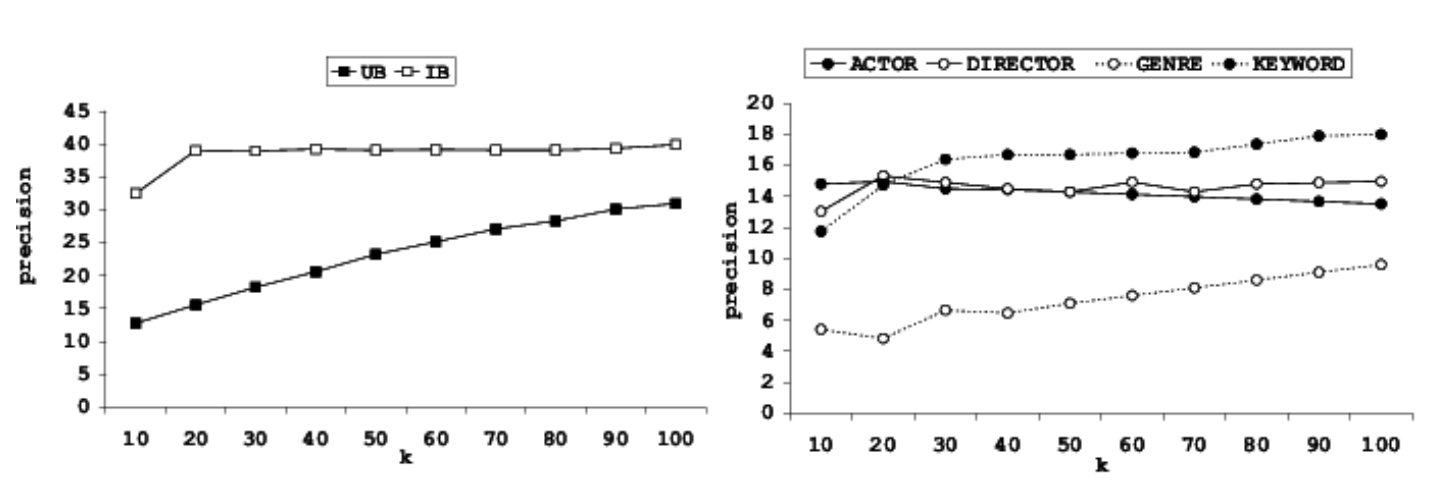
\includegraphics[scale=0.5]{images/comparison2.png}
\end{center}

\end{frame}

\begin{frame}{CF Flavors}

\begin{center}
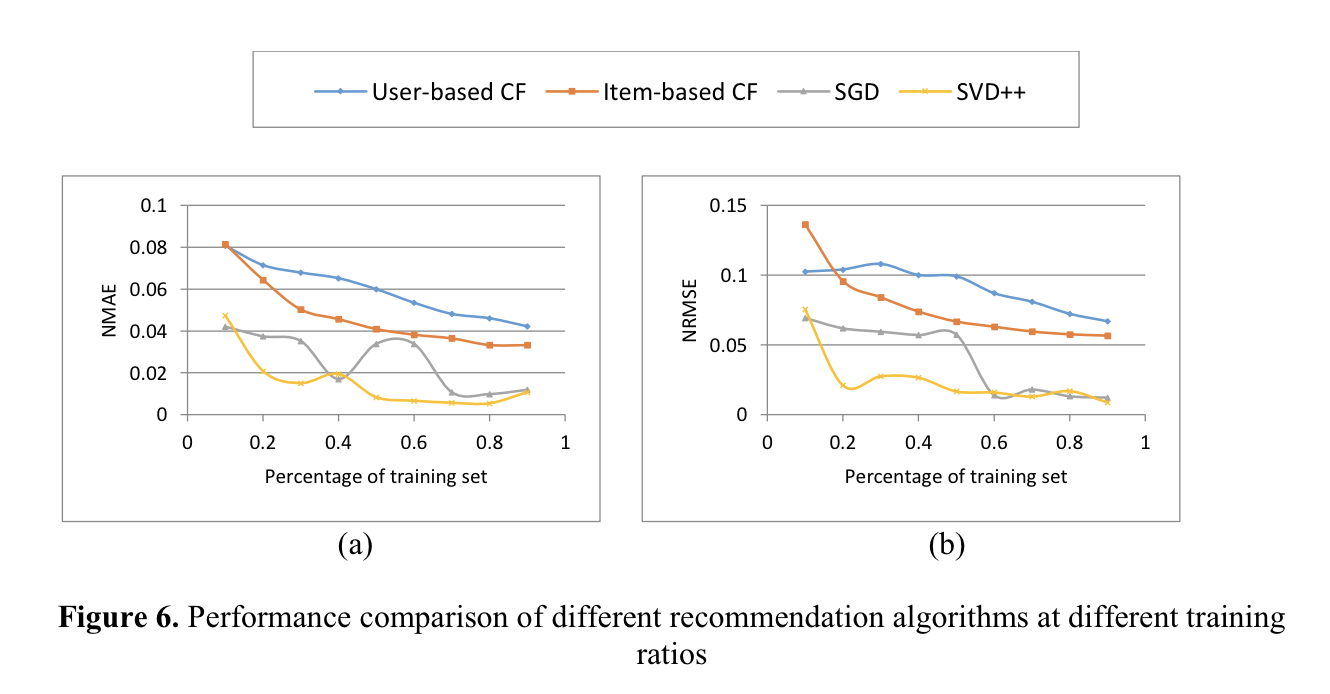
\includegraphics[scale=0.5]{images/comparison.png}
\end{center}

\end{frame}

\begin{frame}

\begin{tcolorbox}[colback=info!5,colframe=info!80,title=]
Реальные рекомендеры почти всегда hybrid: применяются как CF, так и CB подходы
\end{tcolorbox}

\begin{tcolorbox}[colback=info!5,colframe=info!80,title=]
``Дефолтным'' алгоритмом рекомендаций считается матричная факторизация
\end{tcolorbox}

\end{frame}

\begin{frame}{В следующий раз}

\begin{columns}

\begin{column}{0.47\textwidth} 
\begin{center}
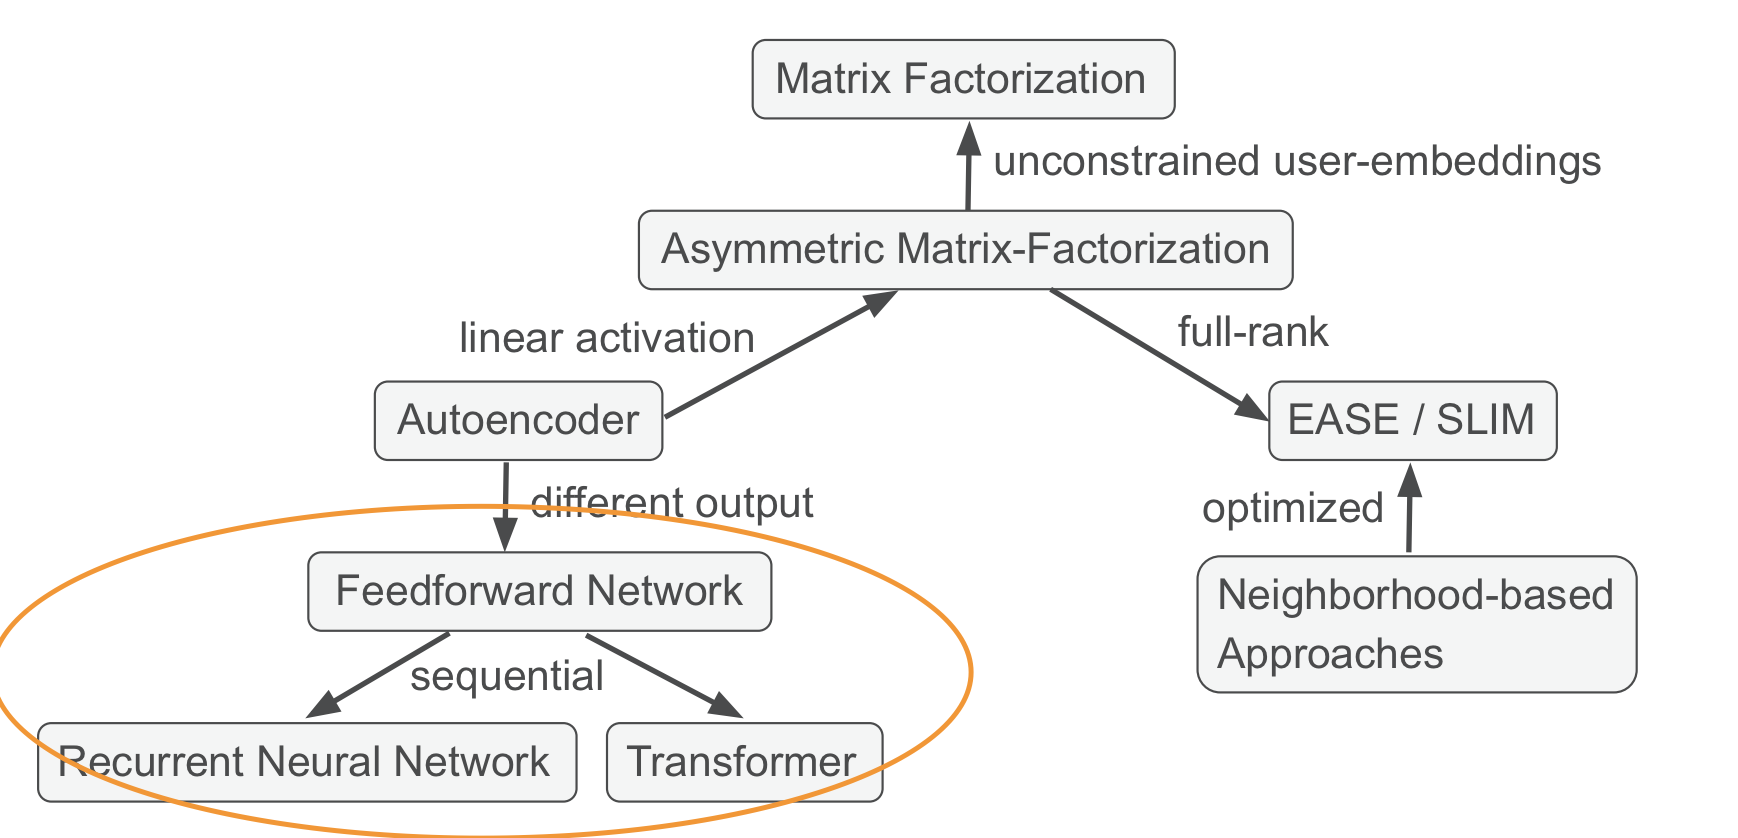
\includegraphics[scale=0.3]{images/relationships.png}
\end{center}
\end{column}

\begin{column}{0.47\textwidth}
\begin{center}

\includegraphics[scale=0.15]{images/conspiracy.jpeg}
\end{center}
\end{column}

\end{columns}

\end{frame}

\begin{frame}[allowframebreaks]{Литература}

\bibliographystyle{amsalpha}
\bibliography{references.bib}

\end{frame}

\end{document}
